\section{密度比较}
\label{sec:dcomp-density}

总变差只用到密度之差$\lvert p-q\rvert$。看两个位置：一处$p=0.02$，$q=0.01$；另一处$p=0.51$，$q=0.50$。两处的差都是$0.01$，对总变差的贡献相同。可是若用$Q$去预测按$P$产生的结果，第一处的结果实际出现的频率是$Q$所说的两倍，第二处只多了百分之二。比值$p(x)/q(x)$记录的正是这种相对失衡。

本节在同一个支配测度$\lambda$下比较同一位置上的两个密度，用对数比、平方根和幂次构造几种比较量，再把它们归入同一个机制：对密度比施加一个凸函数，再求平均。密度为零的位置需要单独约定，而且多数比较量不对称或不满足三角不等式，所以统称为散度，只有满足距离公理的才称为距离。

\subsection{KL散度}
\label{sec:dcomp-kl}

\paragraph{对数比的平均}
设观测到一个结果$x$，要判断它更像来自$P$还是$Q$。比值$p(x)/q(x)$大于$1$时支持$P$，取对数后$\ln(p(x)/q(x))$大于零。对数的好处是独立观测的证据可以相加：$n$次独立观测的密度比是各次比值的乘积，取对数就成了各次对数比之和。如果数据确实来自$P$，每次观测平均提供的证据是对数比在$P$下的期望。由第~\ref{chap:laws-of-large-numbers}章的强大数律，只要这个期望存在，$n$次观测的总证据除以$n$几乎必然趋于它，所以它衡量的是“$P$为真时，平均每次观测能把$P$与$Q$分开多少”。

对数比在$q(x)=0<p(x)$处是$+\infty$：$P$下可能出现、$Q$却认为不可能的结果，一旦出现就彻底否定$Q$。在$p(x)=0$处，这个点在$P$下不出现，对平均没有贡献。定义据此处理零密度。

\begin{definition}[KL散度]
\label{def:dcomp-kl}
设$p,q$是$P,Q$相对于共同支配测度$\lambda$的密度。若$P\ll Q$，定义$P$相对于$Q$的\term{KL散度}（Kullback--Leibler divergence）为
\begin{equation}
 D_{\mathrm{KL}}(P\Vert Q)=\int_{\{p>0\}}p\ln\frac{p}{q}\,\mathrm{d}\lambda=\mathbb{E}_{P}\Bigl[\ln\frac{\mathrm{d}P}{\mathrm{d}Q}\Bigr] ;
 \label{eq:dcomp-kl-def}
\end{equation}
若$P$不绝对连续于$Q$，定义$D_{\mathrm{KL}}(P\Vert Q)=+\infty$。
\end{definition}

定义里有两件事需要核对。第一，积分有意义。$P\ll Q$时$P(q=0)=0$，被积函数在$\{p>0\}$上$\lambda$几乎处处有限。它的负部只出现在$p<q$处，由$\ln u\leq u-1$，
\[
 \int_{\{0<p<q\}}p\ln\frac{q}{p}\,\mathrm{d}\lambda\leq\int_{\{0<p<q\}}p\Bigl(\frac{q}{p}-1\Bigr)\,\mathrm{d}\lambda\leq\int q\,\mathrm{d}\lambda=1 .
\]
负部的积分有限，所以整个积分在$(-\infty,+\infty]$中有确定的值。第二，结果与$\lambda$无关：$P\ll Q$时比值$p/q$在$P$几乎处处的意义下就是Radon–Nikodym密度$\mathrm{d}P/\mathrm{d}Q$，式~\eqref{eq:dcomp-kl-def}的最后一个表达式里没有$\lambda$。

\begin{theorem}[Gibbs不等式]
\label{thm:dcomp-gibbs}
$D_{\mathrm{KL}}(P\Vert Q)\geq0$，等号成立当且仅当$P=Q$。
\end{theorem}

\begin{proof}
若$P$不绝对连续于$Q$，散度为$+\infty$，结论成立。设$P\ll Q$。在$\{p>0\}$上用$\ln u\leq u-1$（等号仅在$u=1$时成立），取$u=q/p$，
\[
 -D_{\mathrm{KL}}(P\Vert Q)=\int_{\{p>0\}}p\ln\frac{q}{p}\,\mathrm{d}\lambda\leq\int_{\{p>0\}}(q-p)\,\mathrm{d}\lambda=Q(p>0)-1\leq0 .
\]
若等号成立，第一个不等号要求$\lambda$几乎处处在$\{p>0\}$上$q=p$，第二个要求$Q(p>0)=1$，即$Q$在$\{p=0\}$上没有质量。两条合起来就是$p=q$几乎处处，即$P=Q$。
\end{proof}

这个结论称为\term{Gibbs不等式}（Gibbs' inequality）。证明里用的$\ln u\leq u-1$是对数函数位于它在$u=1$处切线下方，即凹性。KL散度非负，是因为在$P$自己的权重下，“用$Q$的概率”平均起来不如“用$P$自己的概率”。

\paragraph{方向不对称}
在例表上逐项计算。点$1$处$p=q$，贡献为零；另外两项是
\[
 0.6\ln\frac{0.6}{0.3}=0.6\ln2,\qquad 0.1\ln\frac{0.1}{0.4}=-0.2\ln2 .
\]
两项相加，
\[
 D_{\mathrm{KL}}(P\Vert Q)=0.4\ln2\approx0.2773 .
\]
交换两表，同样的两个位置贡献$0.3\ln(1/2)=-0.3\ln2$与$0.4\ln4=0.8\ln2$，
\[
 D_{\mathrm{KL}}(Q\Vert P)=0.5\ln2\approx0.3466 .
\]
两个方向的数值不同。单项可以为负（例如点$2$处$p<q$），总和却不为负，这正是Gibbs不等式。图~\ref{fig:dcomp-kl-asymmetry}(a)画出各项的贡献：$D_{\mathrm{KL}}(Q\Vert P)$的大头来自点$2$，那里$Q$有$0.4$的质量而$P$只给$0.1$。

\paragraph{高斯分布}
取$P=\mathcal{N}(\mu_1,\sigma_1^{2})$，$Q=\mathcal{N}(\mu_2,\sigma_2^{2})$。两个密度之比的对数是
\[
 \ln\frac{p(x)}{q(x)}=\ln\frac{\sigma_2}{\sigma_1}-\frac{(x-\mu_1)^{2}}{2\sigma_1^{2}}+\frac{(x-\mu_2)^{2}}{2\sigma_2^{2}} .
\]
在$P$下取期望，$\mathbb{E}_{P}[(X-\mu_1)^{2}]=\sigma_1^{2}$，而
\[
 \mathbb{E}_{P}\bigl[(X-\mu_2)^{2}\bigr]=\sigma_1^{2}+(\mu_1-\mu_2)^{2} .
\]
代入得到
\begin{equation}
 D_{\mathrm{KL}}(P\Vert Q)=\ln\frac{\sigma_2}{\sigma_1}+\frac{\sigma_1^{2}+(\mu_1-\mu_2)^{2}}{2\sigma_2^{2}}-\frac12 .
 \label{eq:dcomp-kl-gauss}
\end{equation}
方差相同时它化为$(\mu_1-\mu_2)^{2}/(2\sigma^{2})$，两个方向相等。尺度不同时不对称。图~\ref{fig:dcomp-kl-asymmetry}(b)固定$P=\mathcal{N}(0,1)$，令$Q_s=\mathcal{N}(0,s^{2})$。$s<1$时$Q_s$比$P$窄，$P$在两侧尾部的质量落在$Q_s$密度极小的地方，$D_{\mathrm{KL}}(P\Vert Q_s)$迅速增大；反过来，$D_{\mathrm{KL}}(Q_s\Vert P)$在$s<1$时保持较小。KL散度惩罚的是：参考分布$Q$在$P$有质量的地方给出太小的概率。

\begin{BookInlineFigure}
 \centering
 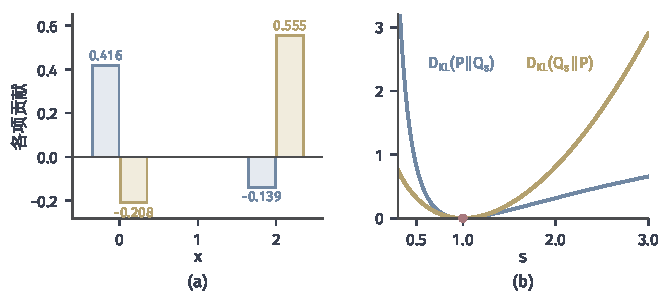
\includegraphics[width=112mm]{figures/07-probability/04-distribution-analysis/matplotlib/dcomp-kl-asymmetry/figure.pdf}
 \caption{KL散度的方向。(a)例表中各点的贡献：蓝色为$p\ln(p/q)$，合计$0.4\ln2\approx0.2773$；黄色为$q\ln(q/p)$，合计$0.5\ln2\approx0.3466$。(b)$P=\mathcal{N}(0,1)$，$Q_s=\mathcal{N}(0,s^{2})$，蓝线为$D_{\mathrm{KL}}(P\Vert Q_s)$，黄线为$D_{\mathrm{KL}}(Q_s\Vert P)$，红点是$s=1$。}
 \label{fig:dcomp-kl-asymmetry}
\end{BookInlineFigure}

\paragraph{绝对连续不保证有限}
$P\ll Q$只排除了“$Q$认为不可能、$P$却可能”的事件，并不保证对数比的平均有限。取$P$为标准Cauchy分布，$Q=\mathcal{N}(0,1)$。两个密度处处为正，互相绝对连续。对数比为
\[
 \ln\frac{p(x)}{q(x)}=\frac{x^{2}}{2}-\ln\bigl(1+x^{2}\bigr)+\ln\sqrt{\frac{2}{\pi}} .
\]
当$\lvert x\rvert$足够大时，右边不小于$x^{2}/4$，而Cauchy分布下$\mathbb{E}_{P}[X^{2}]=+\infty$，所以$D_{\mathrm{KL}}(P\Vert Q)=+\infty$。反方向的散度是对数比的相反数在$\mathcal{N}(0,1)$下的期望，其中$X^{2}$与$\ln(1+X^{2})$都可积，所以$D_{\mathrm{KL}}(Q\Vert P)$有限。用尾部很轻的高斯分布去预测重尾的Cauchy结果，代价是无穷大；反过来则不然。

\subsection{Hellinger距离}
\label{sec:dcomp-hellinger}

KL散度不对称，可以是无穷大，并且对零密度极为敏感。若想要一个真正的距离，可以先把密度开平方。$\sqrt{p}$满足$\int(\sqrt{p})^{2}\,\mathrm{d}\lambda=1$，即它是$L^{2}(\lambda)$中的单位向量。于是每个分布对应单位球面上的一个点，两个分布之间可以用这两个点的欧氏距离比较。

\begin{definition}[Hellinger距离与Bhattacharyya系数]
\label{def:dcomp-hellinger}
设$p,q$是$P,Q$相对于共同支配测度$\lambda$的密度。称
\begin{equation}
 d_{\mathrm{H}}(P,Q)=\frac{1}{\sqrt2}\bigl\lVert\sqrt{p}-\sqrt{q}\bigr\rVert_{L^{2}(\lambda)}=\Bigl(\frac12\int\bigl(\sqrt{p}-\sqrt{q}\bigr)^{2}\,\mathrm{d}\lambda\Bigr)^{1/2}
 \label{eq:dcomp-hellinger-def}
\end{equation}
为\term{Hellinger距离}（Hellinger distance），称
\begin{equation}
 B(P,Q)=\int\sqrt{pq}\,\mathrm{d}\lambda
 \label{eq:dcomp-bhattacharyya-coefficient}
\end{equation}
为\term{Bhattacharyya系数}（Bhattacharyya coefficient）。
\end{definition}

把式~\eqref{eq:dcomp-hellinger-def}中的平方展开，两个密度的积分都是$1$，交叉项正是$B$：
\begin{equation}
 d_{\mathrm{H}}^{2}(P,Q)=\frac12\int\bigl(p+q-2\sqrt{pq}\bigr)\,\mathrm{d}\lambda=1-B(P,Q) .
 \label{eq:dcomp-hellinger-bc}
\end{equation}
由Cauchy--Schwarz不等式，$B$不超过$\sqrt{p}$与$\sqrt{q}$的$L^{2}$范数之积，即$1$；又$B\geq0$，所以$0\leq d_{\mathrm{H}}\leq1$。$d_{\mathrm{H}}=1$当且仅当$B=0$，即$pq=0$几乎处处，两个分布相互奇异。系数$1/\sqrt2$正是为了让最大值等于$1$。$d_{\mathrm{H}}$是$L^{2}(\lambda)$中两个向量之差的范数乘以常数，所以对称并满足三角不等式；$d_{\mathrm{H}}=0$表示$\sqrt{p}=\sqrt{q}$几乎处处，即$P=Q$。它是一个距离。

\paragraph{与支配测度无关}
定义用到了$\lambda$，需要检查换一个支配测度结果不变。设$\lambda$与$\lambda'$都支配$P,Q$。令$\nu=\lambda+\lambda'$，则$\lambda\ll\nu$，记$r=\mathrm{d}\lambda/\mathrm{d}\nu$。由密度的链式法则，$P,Q$相对于$\nu$的密度是$pr$与$qr$，于是
\[
 \int\sqrt{(pr)(qr)}\,\mathrm{d}\nu=\int\sqrt{pq}\,r\,\mathrm{d}\nu=\int\sqrt{pq}\,\mathrm{d}\lambda .
\]
所以用$\lambda$与用$\nu$算出的$B$相同。对$\lambda'$同样推理，三者一致。由式~\eqref{eq:dcomp-hellinger-bc}，$d_{\mathrm{H}}$也与支配测度无关。关键在于$\sqrt{pq}$关于密度是“一次齐次”的：密度整体乘以$r$，它也恰好乘以$r$，与积分测度的变化抵消。

\paragraph{例表与几何图景}
在例表上，
\[
 B(P,Q)=\sqrt{0.18}+\sqrt{0.09}+\sqrt{0.04}\approx0.4243+0.3+0.2=0.9243 .
\]
于是$d_{\mathrm{H}}^{2}\approx0.0757$，$d_{\mathrm{H}}\approx0.2752$。把$\sqrt{p}$与$\sqrt{q}$看成$\mathbb{R}^{3}$中的两个单位向量，$B$是它们的内积，也就是夹角$\theta$的余弦；这里$\theta\approx22.5^{\circ}$。$\sqrt2\,d_{\mathrm{H}}$是两个向量端点之间的弦长，见图~\ref{fig:dcomp-hellinger-roots}(b)。

\paragraph{两个高斯分布}
取方差同为$\sigma^{2}$、均值分别为$\mu_1,\mu_2$的两个高斯分布，记作$P$与$Q$，并记
\[
 \Delta=\mu_1-\mu_2,\qquad m=\tfrac12(\mu_1+\mu_2) .
\]
配方得到
\[
 (x-\mu_1)^{2}+(x-\mu_2)^{2}=2(x-m)^{2}+\frac{\Delta^{2}}{2} .
\]
代入两个密度的乘积再开方，$\sqrt{p(x)q(x)}$是以$m$为中心、方差为$\sigma^{2}$的高斯密度乘以常数
\[
 \exp\Bigl(-\frac{\Delta^{2}}{8\sigma^{2}}\Bigr) .
\]
高斯密度积分为$1$，于是
\begin{equation}
 B(P,Q)=\exp\Bigl(-\frac{(\mu_1-\mu_2)^{2}}{8\sigma^{2}}\Bigr) .
 \label{eq:dcomp-bc-gauss}
\end{equation}
图~\ref{fig:dcomp-hellinger-roots}(a)取$\sigma=1$，$\Delta=1.5$，浅蓝区域的面积是$B=\mathrm{e}^{-9/32}\approx0.7548$。重叠函数$\sqrt{pq}$的峰在两个均值的中点，两个分布离得越远，峰越低。

\begin{BookInlineFigure}
 \centering
 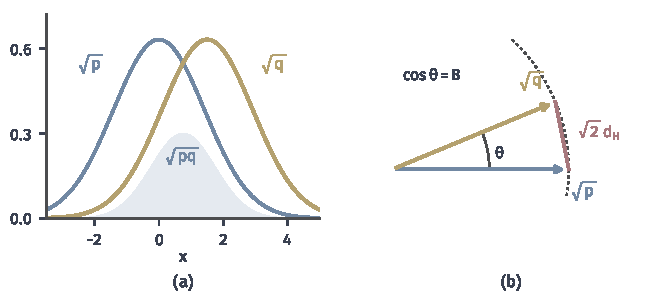
\includegraphics[width=112mm]{figures/07-probability/04-distribution-analysis/matplotlib/dcomp-hellinger-roots/figure.pdf}
 \caption{平方根密度。(a)$P=\mathcal{N}(0,1)$与$Q=\mathcal{N}(1.5,1)$的$\sqrt{p}$（蓝）与$\sqrt{q}$（黄），浅蓝区域是$\sqrt{pq}$，面积为$B\approx0.7548$。(b)例表的$\sqrt{\bm{p}}$与$\sqrt{\bm{q}}$是$\mathbb{R}^{3}$中的单位向量，画在它们张成的平面里；夹角$\theta\approx22.5^{\circ}$，$\cos\theta=B\approx0.9243$，红色弦长为$\sqrt2\,d_{\mathrm{H}}\approx0.389$。}
 \label{fig:dcomp-hellinger-roots}
\end{BookInlineFigure}

\paragraph{Bhattacharyya距离}
重叠系数的负对数
\begin{equation}
 D_{\mathrm{B}}(P,Q)=-\ln B(P,Q)
 \label{eq:dcomp-bhattacharyya-distance}
\end{equation}
称为\term{Bhattacharyya距离}（Bhattacharyya distance）。两个分布相互奇异时$B=0$，它等于$+\infty$，而$d_{\mathrm{H}}$此时只是$1$。$B$接近$1$时，$-\ln B\approx1-B=d_{\mathrm{H}}^{2}$。尽管名字里有“距离”，它不满足三角不等式。由式~\eqref{eq:dcomp-bc-gauss}，方差为$1$、均值分别为$0,1,2$的三个高斯分布两两之间的值是$\Delta^{2}/8$，于是
\[
 D_{\mathrm{B}}(\mathcal{N}(0,1),\mathcal{N}(2,1))=\frac12>\frac18+\frac18 .
\]
它随均值差平方增长，跨两步比走一步再走一步还“远”。在本章的用法里，$B$是重叠系数，$d_{\mathrm{H}}$是距离，$D_{\mathrm{B}}$只是$B$的一个单调变换。

\subsection{JS散度}
\label{sec:dcomp-js}

KL散度要求一个分布绝对连续于另一个。取$P=\operatorname{Unif}(0,1)$，$Q=\operatorname{Unif}(\tfrac12,\tfrac32)$，两个分布有一半质量重叠，可两个方向的KL散度都是$+\infty$：$P$在$(0,\tfrac12)$上有质量而$Q$没有，$Q$在$(1,\tfrac32)$上有质量而$P$没有。问题出在参考分布覆盖不到对方。一个自然的修补是换一个同时覆盖双方的参考分布，最简单的选择是两者的平均
\[
 M=\tfrac12(P+Q) .
\]
$M$的密度是$(p+q)/2$，只要$p>0$或$q>0$，它就为正。

\begin{definition}[JS散度]
\label{def:dcomp-js}
设$M=(P+Q)/2$。$P$与$Q$之间的\term{JS散度}（Jensen--Shannon divergence）是
\begin{equation}
 D_{\mathrm{JS}}(P,Q)=\frac12D_{\mathrm{KL}}(P\Vert M)+\frac12D_{\mathrm{KL}}(Q\Vert M) .
 \label{eq:dcomp-js-def}
\end{equation}
\end{definition}

用密度写出来，$\mathrm{d}P/\mathrm{d}M=2p/(p+q)$，所以
\[
 D_{\mathrm{JS}}(P,Q)=\frac12\int\Bigl(p\ln\frac{2p}{p+q}+q\ln\frac{2q}{p+q}\Bigr)\,\mathrm{d}\lambda ,
\]
其中$p=0$或$q=0$的项按$0\ln0=0$理解。

\begin{theorem}[JS散度的范围]
\label{thm:dcomp-js-range}
$D_{\mathrm{JS}}$对称，并且
\begin{equation}
 0\leq D_{\mathrm{JS}}(P,Q)\leq\ln2 .
 \label{eq:dcomp-js-range}
\end{equation}
左边等号成立当且仅当$P=Q$，右边等号成立当且仅当$P$与$Q$相互奇异。
\end{theorem}

\begin{proof}
交换$P,Q$不改变$M$，式~\eqref{eq:dcomp-js-def}的两项互换，所以对称。$P\ll M$与$Q\ll M$总成立，两项都有定义；由Gibbs不等式，两项都非负。和为零当且仅当两项都为零，即$P=M=Q$。

在$\{p>0\}$上，$2p/(p+q)\leq2$，所以
\[
 D_{\mathrm{KL}}(P\Vert M)=\int_{\{p>0\}}p\ln\frac{2p}{p+q}\,\mathrm{d}\lambda\leq\ln2,
\]
等号成立当且仅当在$\{p>0\}$上$q=0$几乎处处，即$Q(p>0)=0$。对$D_{\mathrm{KL}}(Q\Vert M)$同理，它等于$\ln2$当且仅当$P(q>0)=0$。两项都取到$\ln2$，恰好是$P$集中在$\{q=0\}$上、$Q$集中在$\{p=0\}$上，即两者相互奇异。
\end{proof}

上界$\ln2$有一个直观解释。把$P$与$Q$各以概率$\tfrac12$选出来，再按所选分布产生结果$x$，那么$x$的分布正是$M$。$D_{\mathrm{JS}}$衡量的是看到$x$后能把“选了哪一个”猜得多准；两个分布相互奇异时，看到$x$就知道答案，这一次是非题的全部不确定性$\ln2$都被消除了。这一解释将在第~\ref{chap:information-measures}章用互信息说清。

\paragraph{几个例子}
在例表上，$M=(0.45,\,0.3,\,0.25)$。两项分别是
\[
 D_{\mathrm{KL}}(P\Vert M)=0.6\ln\frac{0.6}{0.45}+0.1\ln\frac{0.1}{0.25}\approx0.0810,
\]
\[
 D_{\mathrm{KL}}(Q\Vert M)=0.3\ln\frac{0.3}{0.45}+0.4\ln\frac{0.4}{0.25}\approx0.0664 .
\]
平均得到$D_{\mathrm{JS}}(P,Q)\approx0.0737$，比上界$\ln2\approx0.6931$小得多。对开头的两个均匀分布，在重叠的$(\tfrac12,1)$上$p=q$，被积函数为零；在$(0,\tfrac12)$上只有$p=1$，被积函数是$\ln2$；在$(1,\tfrac32)$上只有$q=1$，同样是$\ln2$。于是
\[
 D_{\mathrm{JS}}(P,Q)=\frac12\Bigl(\frac12\ln2+\frac12\ln2\Bigr)=\frac12\ln2\approx0.3466 ,
\]
两个方向的KL散度都是$+\infty$，JS散度却是一个有限的数。

图~\ref{fig:dcomp-js-saturation}比较$P=\mathcal{N}(0,1)$与$Q=\mathcal{N}(\Delta,1)$。由式~\eqref{eq:dcomp-kl-gauss}，$D_{\mathrm{KL}}(P\Vert Q)=\Delta^{2}/2$，随$\Delta$无限增长；JS散度在$\Delta$较大时贴近$\ln2$，两个分布几乎不重叠以后，再拉远也几乎不再增加。JS散度有界的代价是：它分不清“已经几乎分开”与“分得非常开”。

\begin{BookInlineFigure}
 \centering
 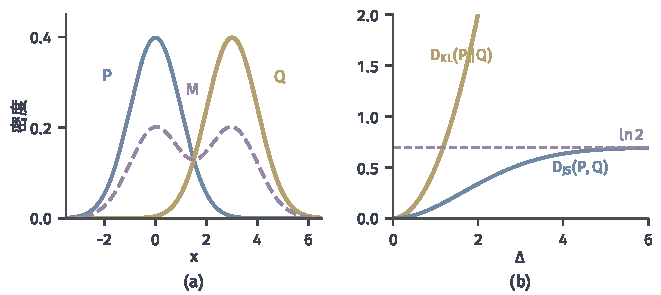
\includegraphics[width=112mm]{figures/07-probability/04-distribution-analysis/matplotlib/dcomp-js-saturation/figure.pdf}
 \caption{JS散度的饱和。(a)$P=\mathcal{N}(0,1)$（蓝）、$Q=\mathcal{N}(3,1)$（黄）与平均分布$M$（紫色虚线）。(b)$D_{\mathrm{KL}}(P\Vert Q)=\Delta^{2}/2$（黄）与$D_{\mathrm{JS}}(P,Q)$（蓝，数值积分），紫色虚线是上界$\ln2$；$\Delta=1,3,6$时JS散度依次约为$0.111$，$0.527$，$0.689$。}
 \label{fig:dcomp-js-saturation}
\end{BookInlineFigure}

\paragraph{距离性质}
JS散度对称、非负、零值只在两分布相同时取到，但它本身不满足三角不等式。在$\{0,1\}$上取$\delta_0$、$\delta_1$与均匀分布$U=(\tfrac12,\tfrac12)$。$\delta_0$与$\delta_1$相互奇异，JS散度取最大值$\ln2\approx0.6931$。$\delta_0$与$U$的平均是$(\tfrac34,\tfrac14)$，计算得
\[
 D_{\mathrm{JS}}(\delta_0,U)=\frac12\ln\frac43+\frac12\Bigl(\frac12\ln\frac23+\frac12\ln2\Bigr)=\frac34\ln\frac43\approx0.2158 .
\]
由对称性$D_{\mathrm{JS}}(U,\delta_1)$也约为$0.2158$，两者之和$0.4315$小于$0.6931$。可以证明$\sqrt{D_{\mathrm{JS}}}$满足三角不等式，因而是一个距离；证明需要把它写成某个Hilbert空间中两点的距离，篇幅较长。上例中$\sqrt{0.2158}\times2\approx0.929$，确实大于$\sqrt{0.6931}\approx0.833$。

\subsection{凸函数散度}
\label{sec:dcomp-f-divergence}

把前面几个量都写成“$Q$下对密度比的某个函数求平均”，会看到同一个形式。在$\{q>0\}$上记$t=p/q$，则
\[
 \frac12\lvert p-q\rvert=q\cdot\frac12\lvert t-1\rvert,\qquad p\ln\frac{p}{q}=q\cdot t\ln t,\qquad\frac12\bigl(\sqrt{p}-\sqrt{q}\bigr)^{2}=q\cdot\frac12\bigl(\sqrt{t}-1\bigr)^{2} .
\]
总变差、KL散度与平方Hellinger距离分别是$\int q\,f(p/q)\,\mathrm{d}\lambda$，$f$依次取$\tfrac12\lvert t-1\rvert$，$t\ln t$与$\tfrac12(\sqrt{t}-1)^{2}$。这三个函数都是凸函数，并且在$t=1$处为零，见图~\ref{fig:dcomp-f-generators}。

\begin{definition}[$f$散度]
\label{def:dcomp-f-divergence}
设$f:(0,\infty)\to\mathbb{R}$是凸函数，$f(1)=0$，并令$f(0)$为极限$\lim_{t\downarrow0}f(t)$，它可以是$+\infty$。若$P\ll Q$，定义
\begin{equation}
 D_f(P\Vert Q)=\mathbb{E}_{Q}\Bigl[f\Bigl(\frac{\mathrm{d}P}{\mathrm{d}Q}\Bigr)\Bigr]=\int_{\{q>0\}}q\,f\Bigl(\frac{p}{q}\Bigr)\,\mathrm{d}\lambda ,
 \label{eq:dcomp-f-def}
\end{equation}
称为$P$相对于$Q$的\term{$f$散度}（$f$-divergence），$f$称为它的生成函数。
\end{definition}

积分有意义：凸函数位于它的任何一条支撑线之上，存在常数$a,b$使$f(t)\geq a+bt$，所以$f(\mathrm{d}P/\mathrm{d}Q)$的负部不超过$\lvert a\rvert+\lvert b\rvert\,\mathrm{d}P/\mathrm{d}Q$，在$Q$下可积。非负性来自Jensen不等式：$\mathbb{E}_{Q}[\mathrm{d}P/\mathrm{d}Q]=1$，所以
\[
 D_f(P\Vert Q)\geq f\Bigl(\mathbb{E}_{Q}\Bigl[\frac{\mathrm{d}P}{\mathrm{d}Q}\Bigr]\Bigr)=f(1)=0 .
\]
凸性在这里起的作用，与Gibbs不等式中对数的凹性相同。

\paragraph{奇异质量}
$P$不绝对连续于$Q$时，$P$在$\{q=0\}$上有质量，那里的密度比相当于$t=+\infty$。从$\{q>0\}$一侧看，$q\,f(p/q)=p\cdot f(t)/t$，当$q\to0$而$p$固定时，它趋于$p\,f'(\infty)$，其中
\begin{equation}
 f'(\infty)=\lim_{t\to\infty}\frac{f(t)}{t}\in\mathbb{R}\cup\{+\infty\} .
 \label{eq:dcomp-f-slope-infinity}
\end{equation}
凸函数的$f(t)/t$在$t$大时单调，这个极限存在。据此把一般情形定义为
\begin{equation}
 D_f(P\Vert Q)=\int_{\{q>0\}}q\,f\Bigl(\frac{p}{q}\Bigr)\,\mathrm{d}\lambda+f'(\infty)\,P(q=0),
 \label{eq:dcomp-f-general}
\end{equation}
约定$0\cdot(+\infty)=0$。KL散度的$f'(\infty)=+\infty$，只要有奇异质量就是$+\infty$，与定义~\ref{def:dcomp-kl}一致。总变差与平方Hellinger距离的$f'(\infty)=\tfrac12$，奇异质量按一半计入：在$\{q=0\}$上$\tfrac12\lvert p-q\rvert$与$\tfrac12(\sqrt{p}-\sqrt{q})^{2}$都等于$\tfrac12p$，与直接用式~\eqref{eq:dcomp-tv-density}和式~\eqref{eq:dcomp-hellinger-def}计算的结果相同。

表~\ref{tab:dcomp-f-generators}列出常用的生成函数。JS散度也在其中：在$\{q>0\}$上把被积函数写成$q$乘以$t=p/q$的函数即得，$f'(\infty)=\tfrac12\ln2$对应于奇异部分每单位质量贡献$\tfrac12\ln2$。$\chi^{2}$散度$\int(p-q)^{2}/q\,\mathrm{d}\lambda$在例表上等于$0.09/0.3+0+0.09/0.4=0.525$。

\begin{BookInlineTable}
 \centering
 \caption{常用$f$散度的生成函数。}
 \label{tab:dcomp-f-generators}
 \begin{tabular}{lll}
  \toprule
  散度 & $f(t)$ & $f'(\infty)$\\
  \midrule
  $D_{\mathrm{KL}}(P\Vert Q)$ & $t\ln t$ & $+\infty$\\
  $D_{\mathrm{KL}}(Q\Vert P)$ & $-\ln t$ & $0$\\
  $d_{\mathrm{TV}}(P,Q)$ & $\tfrac12\lvert t-1\rvert$ & $\tfrac12$\\
  $d_{\mathrm{H}}^{2}(P,Q)$ & $\tfrac12(\sqrt{t}-1)^{2}$ & $\tfrac12$\\
  $D_{\mathrm{JS}}(P,Q)$ & $\tfrac12\bigl(t\ln\tfrac{2t}{1+t}+\ln\tfrac{2}{1+t}\bigr)$ & $\tfrac12\ln2$\\
  $\chi^{2}(P\Vert Q)$ & $(t-1)^{2}$ & $+\infty$\\
  \bottomrule
 \end{tabular}
\end{BookInlineTable}

\begin{BookInlineFigure}
 \centering
 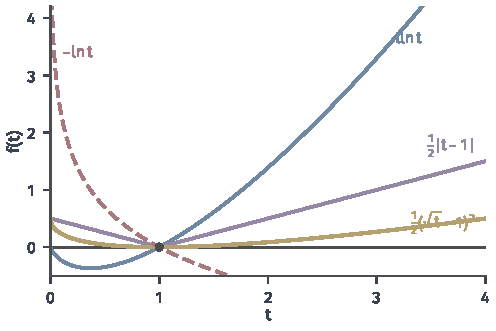
\includegraphics[width=84mm]{figures/07-probability/04-distribution-analysis/matplotlib/dcomp-f-generators/figure.pdf}
 \caption{几个生成函数在$[0,4]$上的图像：$t\ln t$（蓝，KL散度），$-\ln t$（红色虚线，反向KL散度），$\tfrac12\lvert t-1\rvert$（紫，总变差），$\tfrac12(\sqrt{t}-1)^{2}$（黄，平方Hellinger距离）。它们都是凸函数，都经过黑点$(1,0)$；右侧的斜率趋于$f'(\infty)$，决定奇异质量的计价。}
 \label{fig:dcomp-f-generators}
\end{BookInlineFigure}

表中的$-\ln t$与$t\ln t$给出两个方向的KL散度，因为在$Q$下对$-\ln(p/q)$求平均就是$D_{\mathrm{KL}}(Q\Vert P)$。一般地，$t\,f(1/t)$也是凸函数，它生成的散度是$D_f(Q\Vert P)$。生成函数也不唯一：$f(t)$与$f(t)+c(t-1)$给出同一个散度，因为附加项的贡献是$c\bigl(P(q>0)-Q(q>0)\bigr)+c\,P(q=0)=0$。

\paragraph{随机后处理}
设观测值$x$先经过一个随机处理再交给我们：给定$x$，按分布$K(x,\cdot)$产生新的结果$y$。这里$K$是第~\ref{chap:conditional-distributions}章的概率核，可以是确定的映射（$K(x,\cdot)=\delta_{T(x)}$），也可以是加噪声、四舍五入、合并类别。若原来的结果服从$P$，处理后的结果服从
\begin{equation}
 PK(B)=\int K(x,B)\,P(\mathrm{d}x),\qquad B\in\mathcal{F}_{\mathcal{Y}} .
 \label{eq:dcomp-kernel-push}
\end{equation}
直觉上，处理不会凭空增加区分$P$与$Q$的能力：任何能从$y$做出的判断，都可以先自己生成$y$再从$x$做出。下面的定理把这个直觉写成不等式。

\begin{theorem}[后处理不增加$f$散度]
\label{thm:dcomp-data-processing}
设$K$是从$\mathcal{X}$到$\mathcal{Y}$的概率核，$f$满足定义~\ref{def:dcomp-f-divergence}的条件。则
\begin{equation}
 D_f(PK\Vert QK)\leq D_f(P\Vert Q) .
 \label{eq:dcomp-data-processing}
\end{equation}
\end{theorem}

\begin{proof}
下面对$P\ll Q$的情形给出证明，这已经包含了KL散度取有限值的全部情形。若$D_f(P\Vert Q)=+\infty$，结论成立，所以设它有限。记$r=\mathrm{d}P/\mathrm{d}Q$。在一个概率空间上构造$(X,Y)$，使$X\sim Q$，给定$X=x$时$Y$的条件分布是$K(x,\cdot)$，于是$Y\sim QK$。

先找出$PK$相对于$QK$的密度。对$B\in\mathcal{F}_{\mathcal{Y}}$，由式~\eqref{eq:dcomp-kernel-push}与$r$的定义，再对$X$取条件，
\[
 PK(B)=\mathbb{E}\bigl[r(X)K(X,B)\bigr]=\mathbb{E}\bigl[r(X)\mathbf{1}_{\{Y\in B\}}\bigr]=\mathbb{E}\bigl[s(Y)\mathbf{1}_{\{Y\in B\}}\bigr],
\]
其中$s(Y)=\mathbb{E}[r(X)\mid Y]$，最后一步是条件期望的定义；$s$是可测函数，由第~\ref{chap:conditional-expectation}章，条件期望可以写成$Y$的函数。上式说明$PK\ll QK$，并且$s$就是$\mathrm{d}(PK)/\mathrm{d}(QK)$。

于是左边的散度是$\mathbb{E}[f(s(Y))]$。对凸函数$f$用条件Jensen不等式，再用全期望公式，
\[
 \mathbb{E}\bigl[f(\mathbb{E}[r(X)\mid Y])\bigr]\leq\mathbb{E}\bigl[\mathbb{E}[f(r(X))\mid Y]\bigr]=\mathbb{E}\bigl[f(r(X))\bigr]=D_f(P\Vert Q) .
\]
第~\ref{chap:conditional-expectation}章的条件Jensen不等式对定义在$\mathbb{R}$上的凸函数陈述；$f$定义在$[0,\infty)$上，$r\geq0$，证明只用到可数条支撑线，对这里的$f$同样成立。$f(r(X))$可积，因为$D_f(P\Vert Q)$有限且负部可积。
\end{proof}

$P$不绝对连续于$Q$的情形可以用同样的思路证明：取$\lambda=(P+Q)/2$，把两个密度$(\mathrm{d}P/\mathrm{d}\lambda,\mathrm{d}Q/\mathrm{d}\lambda)$一起作为二维随机向量，对二元凸函数$(a,b)\mapsto b\,f(a/b)$使用条件Jensen不等式。步骤与上面相同，只是要另外讨论$b=0$的边界。

证明的核心是一句话：处理后的密度比是处理前密度比的条件平均，而对凸函数先平均再作用，结果不超过先作用再平均。条件平均把不同$x$上的密度比混在一起，比值的起伏被抹平，凸函数度量的“偏离$1$的程度”只能变小。

\paragraph{合并类别}
在例表上做确定的合并。把$1$与$2$合并成一类，两份表变成$(0.6,0.4)$与$(0.3,0.7)$，KL散度从$0.2773$降到
\[
 0.6\ln\frac{0.6}{0.3}+0.4\ln\frac{0.4}{0.7}\approx0.1920 ,
\]
总变差仍是$0.3$。总变差不变，是因为合并后仍能区分最坏事件$A^{*}=\{0\}$。若改把$0$与$2$合并，两份表都变成$(0.7,0.3)$，所有散度都变成零：点$0$处$P$多出的$0.3$与点$2$处$Q$多出的$0.3$被并到同一类里，正好抵消，区分两个分布的信息全部丢失。图~\ref{fig:dcomp-merging}画出这三种情况。

\begin{BookInlineFigure}
 \centering
 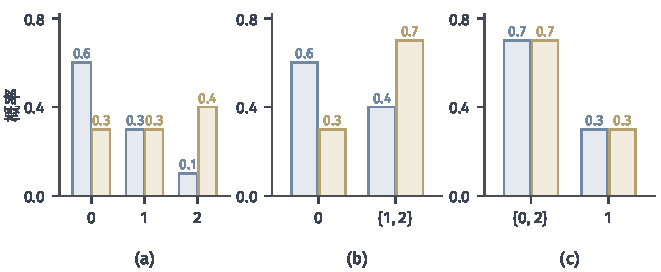
\includegraphics[width=112mm]{figures/07-probability/04-distribution-analysis/matplotlib/dcomp-merging/figure.pdf}
 \caption{确定性后处理对例表的影响，蓝色为$P$，黄色为$Q$。(a)原表：$d_{\mathrm{TV}}=0.3$，$D_{\mathrm{KL}}(P\Vert Q)\approx0.2773$。(b)合并$1$与$2$：$d_{\mathrm{TV}}=0.3$，$D_{\mathrm{KL}}\approx0.1920$。(c)合并$0$与$2$：两表相同，所有散度为零。}
 \label{fig:dcomp-merging}
\end{BookInlineFigure}

若$T$是可测的一一映射且逆映射也可测，对$T$与$T^{-1}$各用一次式~\eqref{eq:dcomp-data-processing}，得到$D_f$在$T$下不变。重新标号、单位换算这类可逆变换不改变任何$f$散度。

\subsection{Rényi散度}
\label{sec:dcomp-renyi}

KL散度按$P$的权重平均对数比。另一种做法是对密度比取幂：在$\{q>0\}$上，
\[
 \int p^{\alpha}q^{1-\alpha}\,\mathrm{d}\lambda=\mathbb{E}_{Q}\Bigl[\Bigl(\frac{p}{q}\Bigr)^{\alpha}\Bigr] .
\]
阶数$\alpha>1$时，幂函数放大大的比值，散度主要由“$P$比$Q$多出很多”的位置决定；$\alpha<1$时放大作用变弱。取对数并归一化，就得到一族以$\alpha$为参数的比较量。

\begin{definition}[Rényi散度]
\label{def:dcomp-renyi}
设$\alpha\in(0,1)\cup(1,\infty)$，$p,q$是相对于共同支配测度$\lambda$的密度。$P$相对于$Q$的$\alpha$阶\term{Rényi散度}（Rényi divergence）是
\begin{equation}
 D_{\alpha}(P\Vert Q)=\frac{1}{\alpha-1}\ln\int p^{\alpha}q^{1-\alpha}\,\mathrm{d}\lambda ,
 \label{eq:dcomp-renyi-def}
\end{equation}
其中被积函数在$p=0$处取$0$；$\alpha>1$时，在$q=0<p$处取$+\infty$。
\end{definition}

零密度的约定决定了无穷值何时出现。$\alpha>1$时，$q^{1-\alpha}$在$q\to0$时趋于无穷，只要$P(q=0)>0$，积分就是$+\infty$，散度为$+\infty$，这与KL散度要求$P\ll Q$一致。$\alpha<1$时，$q^{1-\alpha}\to0$，奇异质量对积分没有贡献；积分为$0$当且仅当$pq=0$几乎处处，即两个分布相互奇异，此时$\ln0=-\infty$除以负数$\alpha-1$，散度同样为$+\infty$。与Hellinger距离一样，被积函数关于密度一次齐次，结果与$\lambda$的选取无关。

两个特殊阶数与前面的量直接对应。$\alpha=\tfrac12$时积分是Bhattacharyya系数，$\alpha=2$时积分是$\int p^{2}/q\,\mathrm{d}\lambda$，它等于$1+\chi^{2}(P\Vert Q)$，所以
\begin{equation}
 D_{1/2}(P\Vert Q)=-2\ln B(P,Q),\qquad D_{2}(P\Vert Q)=\ln\bigl(1+\chi^{2}(P\Vert Q)\bigr) .
 \label{eq:dcomp-renyi-special}
\end{equation}
在例表上，由$B\approx0.9243$与$\chi^{2}=0.525$，
\[
 D_{1/2}\approx0.1575,\qquad D_{\mathrm{KL}}\approx0.2773,\qquad D_{2}=\ln1.525\approx0.4220 .
\]
KL散度恰好夹在中间。图~\ref{fig:dcomp-renyi-order}画出$D_{\alpha}$随$\alpha$的变化，它是一条单调上升的曲线，在$\alpha=1$处连续地经过KL散度。

\begin{BookInlineFigure}
 \centering
 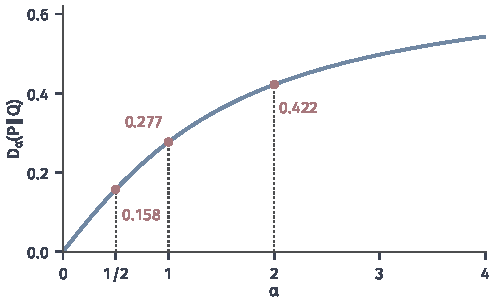
\includegraphics[width=84mm]{figures/07-probability/04-distribution-analysis/matplotlib/dcomp-renyi-order/figure.pdf}
 \caption{例表的Rényi散度$D_{\alpha}(P\Vert Q)$随阶数$\alpha$的变化（蓝）。红点依次是$\alpha=\tfrac12$处的$-2\ln B\approx0.158$，$\alpha=1$处的KL散度$0.4\ln2\approx0.277$，$\alpha=2$处的$\ln(1+\chi^{2})\approx0.422$。}
 \label{fig:dcomp-renyi-order}
\end{BookInlineFigure}

\begin{theorem}[阶数的单调性与KL极限]
\label{thm:dcomp-renyi-order}
对$0<\alpha<1<\beta$，
\begin{equation}
 D_{\alpha}(P\Vert Q)\leq D_{\mathrm{KL}}(P\Vert Q)\leq D_{\beta}(P\Vert Q),
 \label{eq:dcomp-renyi-sandwich}
\end{equation}
并且$\alpha\mapsto D_{\alpha}(P\Vert Q)$在$(0,1)$与$(1,\infty)$上都单调不减，$\alpha\uparrow1$时$D_{\alpha}(P\Vert Q)\to D_{\mathrm{KL}}(P\Vert Q)$。
\end{theorem}

\begin{proof}
若$P$不绝对连续于$Q$，则$D_{\mathrm{KL}}$与所有$\beta>1$的$D_{\beta}$都是$+\infty$，不等式与右侧的单调性成立；左侧的论证不用绝对连续，放在下面一并处理。先设$P\ll Q$。

\emph{改写成幂平均。}在$\{p>0\}$上令$R=q/p$，它在$P$下几乎处处取正的有限值。被积函数在$p=0$处为零，所以
\[
 \int p^{\alpha}q^{1-\alpha}\,\mathrm{d}\lambda=\int_{\{p>0\}}p\,R^{1-\alpha}\,\mathrm{d}\lambda=\mathbb{E}_{P}\bigl[R^{s}\bigr],\qquad s=1-\alpha .
\]
对$s\neq0$记$M_s=(\mathbb{E}_{P}[R^{s}])^{1/s}$，称为$R$的$s$次幂平均，再记$M_0=\exp(\mathbb{E}_{P}[\ln R])$。由式~\eqref{eq:dcomp-renyi-def}与式~\eqref{eq:dcomp-kl-def}，
\[
 D_{\alpha}(P\Vert Q)=-\ln M_{1-\alpha},\qquad D_{\mathrm{KL}}(P\Vert Q)=-\mathbb{E}_{P}[\ln R]=-\ln M_0 .
\]
$\alpha$增大时$s$减小，所以只需证明$M_s$关于$s$单调不减。

\emph{幂平均的单调性。}对$0<s<t$，函数$u\mapsto u^{t/s}$在$[0,\infty)$上凸，由Jensen不等式，
\[
 \bigl(\mathbb{E}_{P}[R^{s}]\bigr)^{t/s}\leq\mathbb{E}_{P}[R^{t}],
\]
开$t$次方得$M_s\leq M_t$。对$s<t<0$，把同一结论用于$1/R$与指数$-t<-s$，取倒数即得。对$s<0<t$，由对数的凹性，
\[
 t\,\mathbb{E}_{P}[\ln R]\leq\ln\mathbb{E}_{P}[R^{t}],\qquad s\,\mathbb{E}_{P}[\ln R]\leq\ln\mathbb{E}_{P}[R^{s}] .
\]
第一式除以$t>0$得$\ln M_0\leq\ln M_t$；第二式除以$s<0$，不等号反向，得$\ln M_0\geq\ln M_s$。于是$M_s\leq M_0\leq M_t$，这就是式~\eqref{eq:dcomp-renyi-sandwich}与两段上的单调性。$\mathbb{E}_{P}[R^{s}]=+\infty$（$s<0$时可能发生）时$M_s=0$，对应的散度为$+\infty$，不等式仍成立。

\emph{左侧的极限。}令$\alpha\uparrow1$，即$s\downarrow0$。对固定的$R>0$，$s\mapsto R^{s}$是凸函数，差商$(R^{s}-1)/s$随$s$减小而单调下降，极限是$\ln R$；$s=1$时差商为$R-1$，在$P$下可积。由单调收敛定理（单调下降、首项可积），
\[
 a_s=\mathbb{E}_{P}\Bigl[\frac{R^{s}-1}{s}\Bigr]\downarrow\mathbb{E}_{P}[\ln R]=-D_{\mathrm{KL}}(P\Vert Q) .
\]
而$\mathbb{E}_{P}[R^{s}]=1+s\,a_s$，所以
\[
 -D_{\alpha}(P\Vert Q)=\frac{1}{s}\ln\mathbb{E}_{P}[R^{s}]=\frac{\ln(1+s\,a_s)}{s} .
\]
若$D_{\mathrm{KL}}$有限，$s\,a_s\to0$，$\ln(1+u)/u\to1$，所以$-D_{\alpha}\to-D_{\mathrm{KL}}$。若$D_{\mathrm{KL}}=+\infty$，由$\ln(1+u)\leq u$得$-D_{\alpha}\leq a_s\to-\infty$。两种情形都有$D_{\alpha}\to D_{\mathrm{KL}}$。

最后，$P$不绝对连续于$Q$时，把$R$在$\{q=0<p\}$上定义为$0$，上面关于$s\in(0,1)$的改写和左侧的极限论证照样成立，结论是$D_{\alpha}\to+\infty=D_{\mathrm{KL}}$。
\end{proof}

\paragraph{另一侧的极限需要条件}
$\alpha\downarrow1$时，$D_{\beta}$未必趋于KL散度。在正整数上取
\[
 p_k=c\,k^{-3},\qquad q_k=(\mathrm{e}-1)\,\mathrm{e}^{-k},\qquad k=1,2,\dots,
\]
其中$c=1/\sum_kk^{-3}\approx0.8319$。对数比$\ln(p_k/q_k)$约按$k$线性增长，而$p_k$按$k^{-3}$衰减，所以$D_{\mathrm{KL}}(P\Vert Q)=\sum_kp_k\ln(p_k/q_k)$收敛，数值约为$0.1446$。但对任何$\beta>1$，
\[
 p_k^{\beta}q_k^{1-\beta}=c^{\beta}(\mathrm{e}-1)^{1-\beta}\,k^{-3\beta}\,\mathrm{e}^{(\beta-1)k}\to+\infty,
\]
级数发散，$D_{\beta}(P\Vert Q)=+\infty$。比值$p_k/q_k$的增长是指数型的，任何正次幂都会让它压过$p_k$的多项式衰减，而对数只把它变成线性增长。若存在某个$\beta>1$使$D_{\beta}$有限，那么$\alpha\downarrow1$时$D_{\alpha}\to D_{\mathrm{KL}}$，证明与上面类似，用支配收敛定理代替单调收敛定理。

\paragraph{与$f$散度的关系}
令$f_{\alpha}(t)=(t^{\alpha}-1)/(\alpha-1)$。$\alpha>1$时$t^{\alpha}$凸，除以正数；$\alpha<1$时$t^{\alpha}$凹，除以负数，所以$f_{\alpha}$总是凸函数，并且$f_{\alpha}(1)=0$。它生成的$f$散度记作$H_{\alpha}$，对比式~\eqref{eq:dcomp-renyi-def}，
\[
 D_{\alpha}(P\Vert Q)=\frac{1}{\alpha-1}\ln\bigl(1+(\alpha-1)H_{\alpha}(P\Vert Q)\bigr) .
\]
右边是$H_{\alpha}$的单调增函数，所以定理~\ref{thm:dcomp-data-processing}立即给出：后处理也不增加Rényi散度。

单调变换保住了大小顺序，却改变了结构，$D_{\alpha}$本身一般不是$f$散度。任何$f$散度在不交区域上按权相加：若$P=\tfrac12P_1+\tfrac12P_2$，$Q=\tfrac12Q_1+\tfrac12Q_2$，并且$P_1,Q_1$集中在$A$上，$P_2,Q_2$集中在$A^{\mathrm{c}}$上，把式~\eqref{eq:dcomp-f-general}的积分拆到$A$与$A^{\mathrm{c}}$上就得到
\[
 D_f(P\Vert Q)=\tfrac12D_f(P_1\Vert Q_1)+\tfrac12D_f(P_2\Vert Q_2) .
\]
在$\{0,1,2\}$上取$A=\{0,1\}$与
\[
 P=(\tfrac12,\ 0,\ \tfrac12),\qquad Q=(\tfrac14,\ \tfrac14,\ \tfrac12) .
\]
按上面的分解，$P_1=(1,0)$与$Q_1=(\tfrac12,\tfrac12)$在$A$上，$P_2,Q_2$都是$\delta_2$。直接计算，
\[
 D_2(P\Vert Q)=\ln\Bigl(\frac{1/4}{1/4}+\frac{1/4}{1/2}\Bigr)=\ln1.5\approx0.4055,
\]
而按块加权的结果是
\[
 \tfrac12D_2(P_1\Vert Q_1)+\tfrac12D_2(P_2\Vert Q_2)=\tfrac12\ln2+0\approx0.3466 .
\]
两者不等，所以不存在$f$使$D_2=D_f$对所有分布对成立。作为对照，KL散度满足这个可加性：$D_{\mathrm{KL}}(P\Vert Q)$与$\tfrac12D_{\mathrm{KL}}(P_1\Vert Q_1)$都等于$\tfrac12\ln2$。
